%! Author = tstreule

\section{Connectionism}\label{sec:connectionism}


%% ===
%\subsection{Perceptron}
%
%The perceptron is a symmetric threshold unit:
%\begin{formula}{Sign unit}
%    $\highlight{(\symbf x, \symbf\theta) \mapsto
%    \mathrm{sign}(\symbf x\cdot \symbf\theta)} =
%    \begin{cases}
%        +1 & \textrm{if } \sum_i x_i\theta_i \geq 0 \\
%        -1 & \textrm{otw.}
%    \end{cases}$
%\end{formula}
%
%Given the labels $y = \pm1$, the perceptron starts at $\symbf\theta \leftarrow \symbf 0$ and \textbf{updates} the weights $\symbf\theta \leftarrow \symbf\theta + \Delta\symbf\theta$ only in case of a mistake.
%\begin{formula}{Perceptron rule}
%    $\Delta\symbf\theta =
%    \begin{cases}
%        \symbf 0 & \textrm{if } y \cdot \mathrm{sign}(\symbf{x\cdot\theta}) \geq 0 \\
%        \highlight{y\symbf x} & \textrm{otw.}
%    \end{cases}$
%\end{formula}


% ===
\subsection{Willshaw memory}

Associative memory, pairs of $(\symbf x^t, \symbf y^t) \in \mathcal S$.\quad Learn $\symbf x^t \mapsto \symbf y^t$:
\begin{formula}{W. learning}
    $\begin{cases}
        \highlight{\Theta_{ji} = \min\brace*{
            1, \sum\nolimits_{t=1}^s y_j^t x_i^t
        }}
        \\
        \Theta^t = \symbf y^t (\symbf x^t)^\top
        \:,\quad
        \Theta = \min\brace*{ \symbf 1, \sum\nolimits_{t=1}^s \Theta^t }
    \end{cases}$
\end{formula}

Since $\Theta^t \symbf x^t = (\symbf x^t \cdot \symbf x^t) y^t = ry^t$, retrieving $y$ for a given $\symbf x$ is:
\begin{formula}{W. retrieval}
    $\symbf x \mapsto \symbf z \mapsto \symbf y, \quad
    \highlight{\symbf z = \Theta \symbf x}, \quad
    \highlight{y_j} = \begin{cases} 0 & z_j < r \\ 1 & \textrm{otw.} \end{cases}$
\end{formula}

\begin{figure}[H]
    \centering
    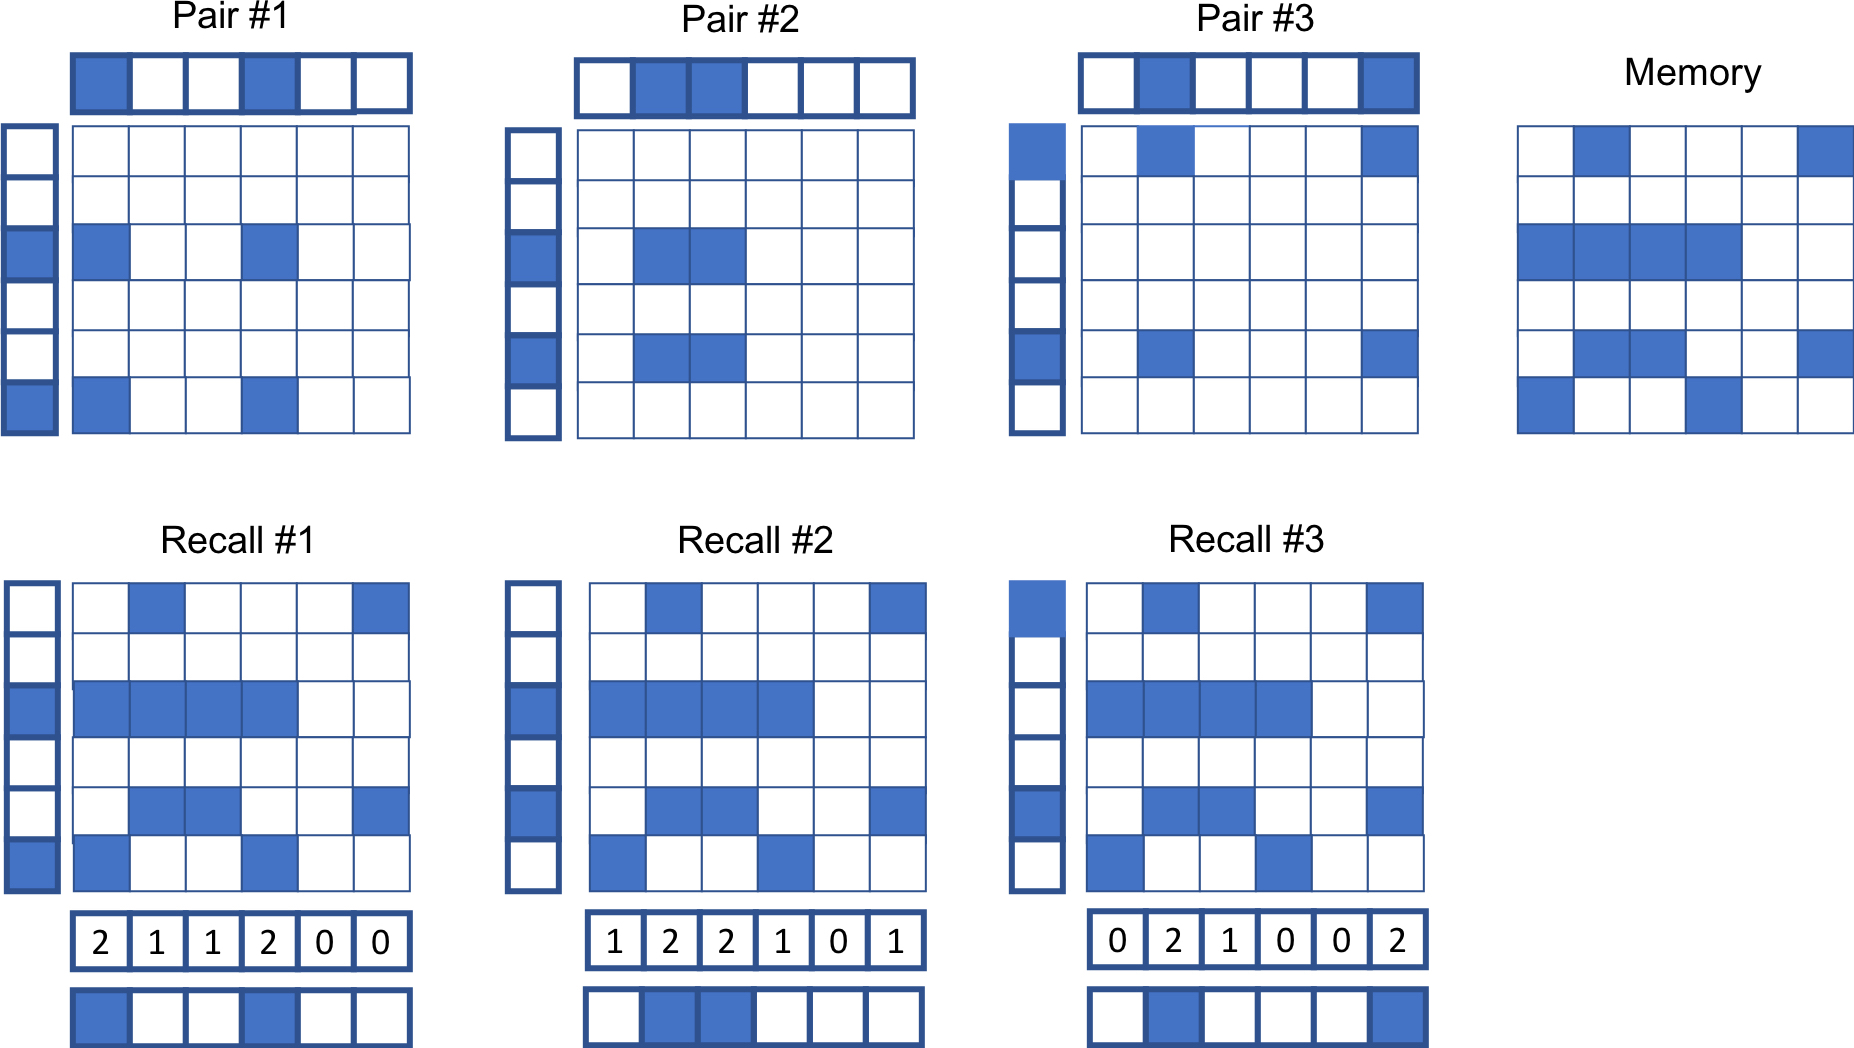
\includegraphics[width=.8\linewidth]{willshaw-memory.jpg}
\end{figure}


% ===
\subsection{Hopfield network}

Assume neurons $x_i \in\brace{-1,1}$ with couplings $\symbf\Theta = (\theta)_{ij}$ such that
\enskip (1) symmetric: \highlight{$\theta_{ij} = \theta_{ji}$}
\enskip (2) irreflexive: \highlight{$\theta_{ii} = 0$}
.

The \textbf{update scheme} is given as follows
\begin{formula}{H. learning}
    $\highlight{x_i \leftarrow \mathrm{sign} \brace*{
        \sum_{j\neq i} \theta_{ij} x_j \green{+ \theta_{i0}}
    }}
    \enspace\green{\text{(bias)}}$
\end{formula}

Convergence is apparent from the Lyapunov equation
\begin{formula}{Ising model}
    $\mathcal E = - \sum\nolimits_{i,j=1}^n \theta_{ij} x_i x_j - \sum\nolimits_{i=1}^n \theta_{i0} x_i$
\end{formula}

Recurr. netw. that can work as \textbf{auto-associative} memory:
\begin{formula}{H. memory}
    $\symbf\Theta \propto \sum\nolimits_{t=1}^s \left[
    \symbf x_t \symbf x_t^\top - \symbf I
    \right] \in \mathbb Z^{n\times n}$
\end{formula}


%% ===
%\subsection{Multilayer perceptron}
%
%\todo{I guess this will come somewhen later...}
